\documentclass[../thesis.tex]{subfiles}
\begin{document}
\chapter{Overview of Organic Semiconductors}

\section{Organic Semiconductors}

\section{Excitons}\label{sec:excitons}
\subsection{Singlets and Triplets}


\begin{wrapfigure}{r}{.5\textwidth}
\centering
\includegraphics[width=.48\textwidth]{orgSemiconductors/jablonski}
\caption{Simplified Jablonski diagram.}
\label{fig:orgSemi_jablonski}
\end{wrapfigure}


\subsection{Electronic Transitions}
\subsection{Quenching Processes}
\subsection{PL efficiency}

\section{Charge Transport}




\ifcsdef{mainfile}{}{\printbibliography}
\end{document}
